\usetikzlibrary{arrows.meta,calc}
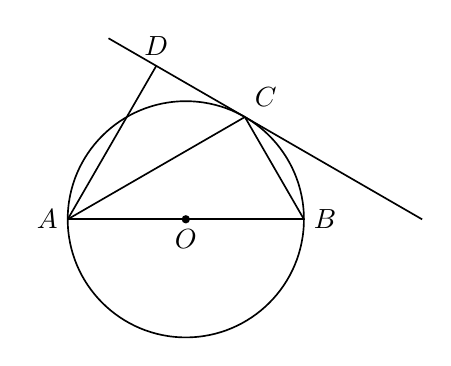
\begin{tikzpicture}[x=1cm,y=1cm,line width=.6pt,font=\normalsize,>=Stealth]
\coordinate (O) at (0,0);
\coordinate (A) at (-1.5,0);
\coordinate (B) at (1.5,0);
\coordinate (C) at (0.75,1.299);
\coordinate (D) at (-0.375,1.9486);
\coordinate (T1) at (-0.982,2.299);
\coordinate (T2) at (3.0016,-0.001);
\draw (O) circle[radius=1.5cm];
\draw (A)--(B);
\draw (A)--(C);
\draw (B)--(C);
\draw (T1)--(T2);
\draw (A)--(D);
\fill (O) circle (1.5pt);
\node[left] at (A) {$A$};
\node[right] at (B) {$B$};
\node[above right] at (C) {$C$};
\node[above] at (D) {$D$};
\node[below] at (O) {$O$};
\end{tikzpicture}
